\chapter{Result}

\section{Methods Comparison Result}

For the methods in Chapter 2, we sorted genes according to the computed measure of the strength of evidence for DE. From these sorted lists, we calculated area under ROC curve (AUC) values to evaluate the ability of these methods to distinguish genes with DE. 

Figure \ref{auc} provides the area under the ROC curve (AUC) across the 5 simulations for each of the scenario defined in \ref{tab:Scenario}. I facetted the plots by number of samples (nSample) and differential gene expression proportion (pDiff), grouped by different level of total number of genes. 

\begin{figure}[h!tb] 
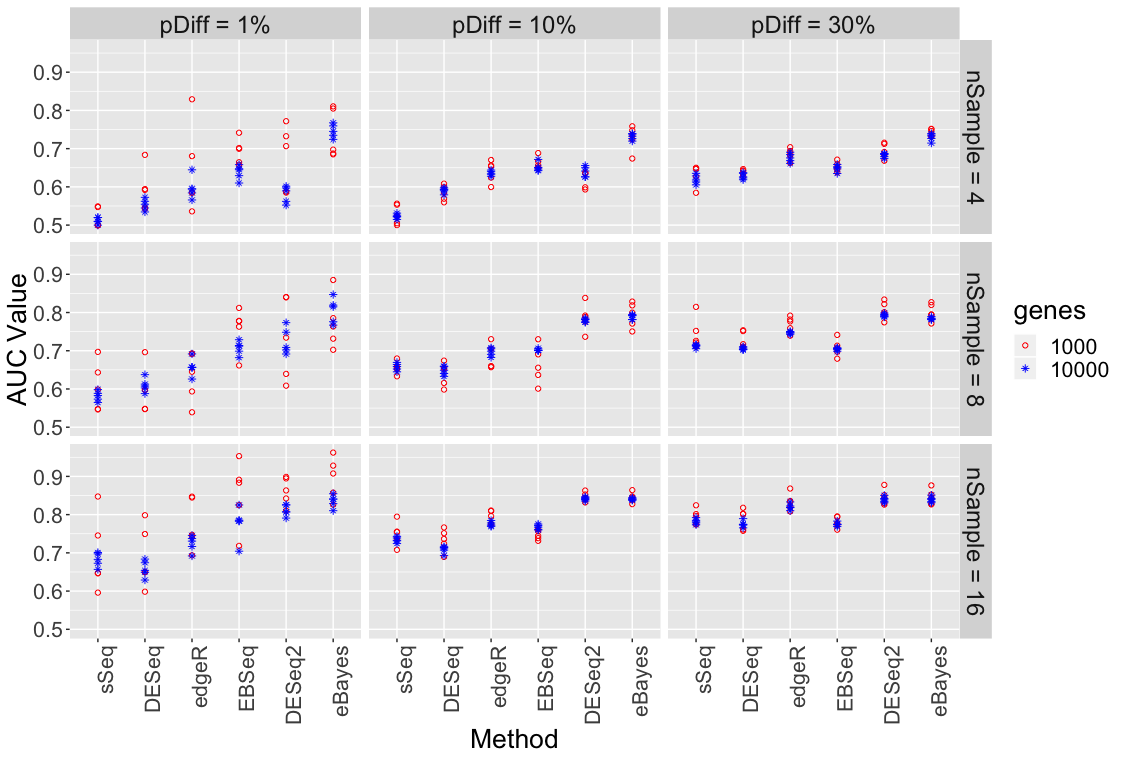
\includegraphics[height=10cm,width=18cm]{auc_plot}
\caption{AUC Plot of Simulated Datasets across Six Methods, Facetted by proportion of DE (pDiff) and number of samples (nSample), Colored by total number of Genes (nGenes)}
\label{auc}
\end{figure}

In terms of AUC values, ebayes method always have promising DE analysis performance.

When number of samples increases, AUC values of all methods increase. 

When DE proportion increases, the difference among the methods decreases. 

There is no obvious difference when number of genes differ.


\section{Discussion}






